\documentclass{article}
\usepackage[utf8]{inputenc}
\usepackage[italian]{babel}
\usepackage{graphicx}
\usepackage{tabu}
\usepackage{booktabs}

\author{Alessandro Righi}
\title{Progetto ingegneria del software}

\begin{document}
\maketitle
\tableofcontents

\section{Introduzione}
Il progetto consiste nella creazione di un prototipo di applicazione per un negozio di CD/DVD musicali. 
Di seguito la specifica del progetto

\subsection{Specifica del progetto}	

Si vuole progettare un sistema informativo per gestire le informazioni relative alla gestione di un negozio
virtuale di CD e DVD musicali (vende solo via web).

Il negozio mette in vendita CD di diversi generi: jazz, rock, classica, latin, folk, world-music, e così via.
Per ogni CD o DVD il sistema memorizza: un codice univoco, il titolo, i titoli di tutti i pezzi contenuti,
eventuali fotografie della copertina, il prezzo, la data dalla quale è presente sul sito web del negozio, il
musicista/band titolare, una descrizione, il genere del CD o DVD, i musicisti che vi suonano, con il
dettaglio degli strumenti musicali usati. Per ogni musicista il sistema registra il nome d’arte, il genere
principale, l’anno di nascita, se noto, gli strumenti che suona.

Sul sito web del negozio è illustrato il catalogo dei prodotti in vendita.
Cliccando sul nome del prodotto, appare una finestra con i dettagli del prodotto stesso.
I clienti possono acquistare on-line selezionando gli oggetti da mettere in un “carrello della spesa”
virtuale.

Deve essere possibile visualizzare il contenuto del carrello, modificare il contenuto del carrello, togliendo
alcuni articoli.

Al termine dell’acquisto va gestito il pagamento, che può avvenire con diverse modalità.

Il sistema supporta differenti ricerche: per genere, per titolare del CD o DVD, per musicista partecipante,
per prezzo. Coerentemente, differenti modalità di visualizzazione, sono altresì supportate.

Ogni vendita viene registrata indicando il cliente che ha acquistato, i prodotti acquistati, il prezzo
complessivo, la data di acquisto, l’ora, l’indirizzo IP del PC da cui è stato effettuato l’acquisto, la modalità
di pagamento (bonifico, carta di credito, paypal) e la modalità di consegna (corriere, posta, …).
Per ogni cliente il sistema registra: il suo codice fiscale, il nome utente (univoco) con cui si è registrato,
la sua password, il nome, il cognome, la città di residenza, il numero di telefono ed eventualmente il
numero di cellulare.

Per i clienti autenticati, il sistema propone pagine specializzate che mostrano suggerimenti basati sul
genere dei precedenti prodotti acquistati.

Se il cliente ha fatto già 3 acquisti superiori ai 250 euro l’uno entro l’anno, il sistema gli propone sconti e
consegna senza spese di spedizione.

Il personale autorizzato del negozio può inserire tutti i dati dei CD e DVD in vendita. Il personale
inserisce anche il numero di pezzi a magazzino. Il sistema tiene aggiornato il numero dei pezzi a
magazzino durante la vendita e avvisa il personale del negozio quando un articolo (CD o DVD) scende
sotto i 2 pezzi presenti in magazzino.	

\section{Analisi dei casi d'uso principali}
\subsection{Use case diagram}
\begin{center}
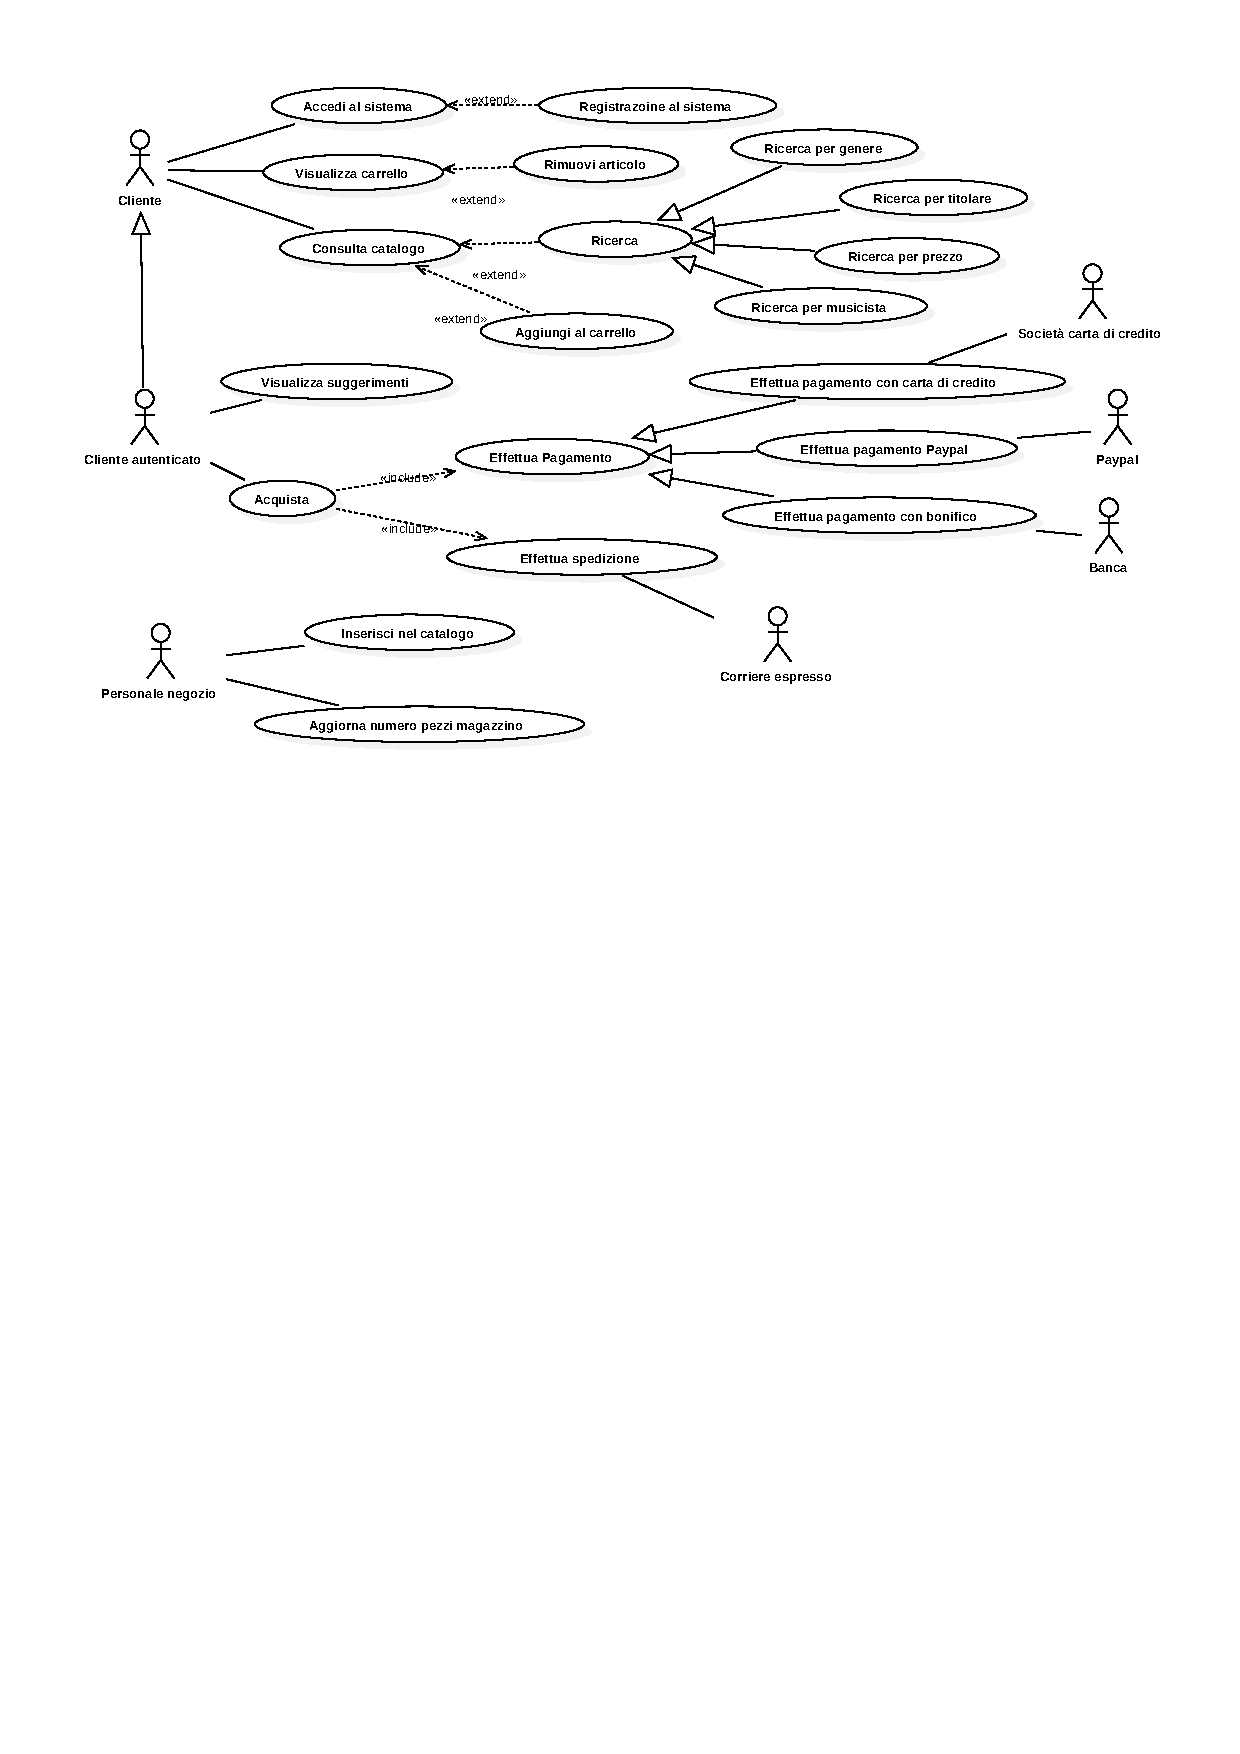
\includegraphics[clip, trim=0.5cm 16cm 0.5cm 0cm, width=1.0\textwidth]{use-case-diagram.pdf}
\end{center}
\subsection{Attori}
Gli attori che interagiscono con il sistema sono i seguenti:
\begin{itemize}
	\item cliente - indica un generico cliente del negozio
	\item cliente autenticato - indica un cliente già autenticato presso il negozio 
	\item presonale negozio - indica un dipendente del negozio
	\item società carta di credito - indica la società che prende parte durante il pagamento con carta di credito
	\item paypal - indica l'attore che prende parte durante il pagamento PayPal
	\item banca - indica la banca che prende parte al pagamento con bonifico
	\item corriere espresso - indica il corriere che prende parte alla spedizione dell'acquisto
\end{itemize}
\subsection{Schede specifica casi d'uso principali} 
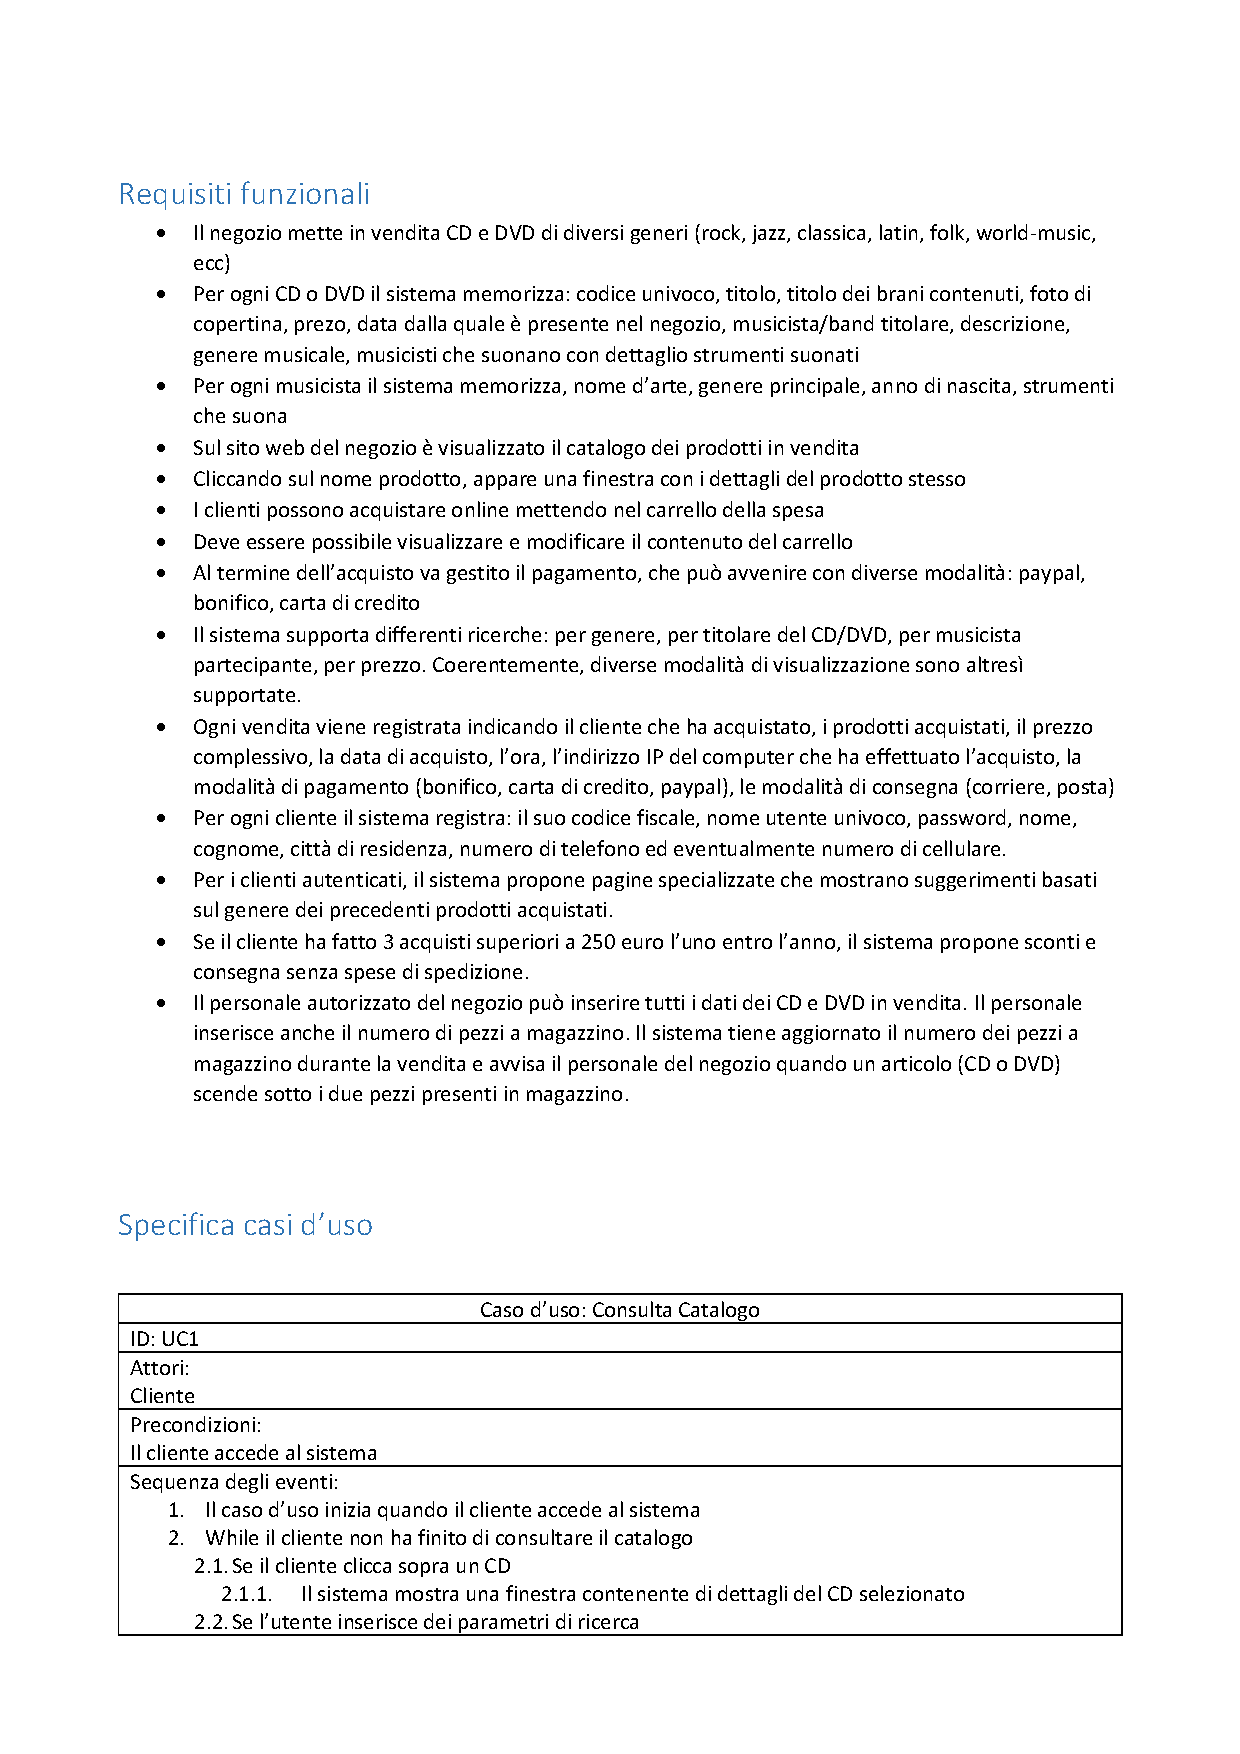
\includegraphics{casi-uso.pdf}
%\section{Sequence diagram dei casi d'uso principali}
%\section{Activity Diagram}

\section{Implementazione del prototipo}
Per l'implementazione del prototipo ho scelto di utilizzare il linguaggio di programmazione Java versione 8, in maniera tale da poter
effettuare una progettazione orientata agli oggetti come richiesto dalla consegna. 

Il prototipo implementa solamente una parte di tutte le funzionalità previste dalle specifiche: in particolare, viene implementata la 
visualizzazione del catalogo del negozio, compresa la ricerca per titolo, genere, autore, musicista e prezzo, la possibilità di
aggiungere o rimuovere CD dal carrello, e l'autenticazione compresa la possibilità di registrare nuovi utenti nel sistema. 

Non viene implementata la procedura di acquisto di un CD, ne la parte relativa all'amministrazione del negozio che consente di modificare
gli oggetti a catalogo o in magazzino. 

Tuttavia la progettazione della base di dati aderisce completamente alle specifiche, sebbene alcune parti non vengono mai utilizzate. 

Per organizzare il progetto ho scelto di utilizzare il sistema VCS git, appoggiandomi alla piattaforma GitHub per l'hosting del 
repository.

\subsection{Interfaccia grafica}
Per la realizzazione dell'interfaccia grafica ho optato per l'utilizzo delle librerie grafiche Swing. Per facilitare l'operazione 
di progetto dell'interfaccia grafica, mi sono avvalso sia del tool di design grafico integrato nell'IDE IntelliJ Idea, sia della 
scrittura manuale di certe parti del codice. 

L'applicazione consiste in una finestra principale, implementata nella classe MainWindow, il cui compito è quello di visualizzare 
il catalogo del negozio e consentire la ricerca, e da varie finestre di dialogo secondarie fra una finestra per visualizzare i dettagli di un album, una per mostrare il carrello, una per effettuare il login e infine una per la registrazione di un nuovo utente. 


\subsection{Base di dati}
Per salvare i dati relativi all'applicazione, ho ritenuto opportuno utilizzare una base di dati esterna. 

Come DBMS ho scelto di utilizzare MySQL versione 5.7. La comunicazione fra Java e il database viene gestita mediante l'interfaccia JDBC grazie alla libreria ufficiale Connector/J fornita dagli sviluppatori di MySQL. 

Lo schema concettuale della base di dati (diagramma ER) è il seguente:
% inserire qui diagramma ER

Lo schema logico della base di dati è invece il seguente:
% inserire schema logico

\subsection{Design pattern utilizzati}
Per lo sviluppo del progetto, ho utilizzato una serie di design pattern.

In primo luogo, il pattern MVC (Model View Controller) che è intrinsecamente usato da Swing. Sebbene nel mio programma view e controller
spesso siano implementati nello stesso file per semplicità del codice, il model, ossia la parte di codice che comunica con la base di 
dati, viene implementata separatamente dalla logica grafica dell'applicazione. 

Per la comunicazione con la base di dati, ho deciso di utilizzare il pattern DAO (Data Access Object), che consente di astrarre la
gestione della base di dati in oggetti standard Java. Il pattern consiste in delle interfacce, per esempio la classe Catalog che
rappresenta il catalogo del negozio e la classe Users che rappresenta il database degli utenti, e la relativa implementazione realizzata 
rispettivamente nelle classi CatalogDatabase e UsersDatabase. 

Questo pattern consente, nel caso si voglia cambiare l'implementazione della base di dati di non dover modificare il codice relativo 
all'interfaccia utente. È anche possibile in questo modo supportare più DBMS diversi nella stessa applicazione, si tratta solamente di 
implementare le interfacce per ogni DBMS che si vuole supportare, e modificare opportunamente la classe Database per consentire la 
scelta fra queste. 

Ho utilizzato infine il pattern Observer, per gestire l'aggiornamento del carrello. Questo consente di registrare un metodo osservatore
che viene chiamato ogni qualvolta che il contenuto del carrello viene modificato, e consente nel caso dell'applicazione la modifica del
conteggio degli oggetti contenuti nel carrello e l'aggiornamento dello stesso. 

Viene infine implementato il pattern Singleton, usato ad esempio dalla classe \textit{Cart}, che rappresenta il carrello. 
Il costruttore della classe è dichiarato private e viene messo a disposizione un metodo \textit{getInstance()} statico 
che ritorna l'istanza dell'oggetto.  

%\section{Class diagram}
%\section{Test del prototipo}
%\section{Conclusioni}
\end{document}